\documentclass[10pt, a4paper]{book}

%\usepackage{amssymb,amsmath}
%\usepackage[a4paper,left=2.7cm,right=3cm]{geometry}
%\usepackage{relsize}
%\usepackage{booktabs}
%\usepackage{graphicx}
\usepackage{hyperref}
%\usepackage{verbatim}
%\usepackage{subfig}
%\usepackage{colortbl}

\def \hsp {\hspace{17mm}}
%
\newcommand\blfootnote[1]{%
  \begingroup
  \renewcommand\thefootnote{}\footnote{\tiny #1}%
  \addtocounter{footnote}{-1}%
  \endgroup
}
%
\newcommand{\pname}[1]{\textnormal{\textsc{#1}}}
\newcommand{\cclass}[1]{\textnormal{\textsf{#1}}}


%\usepackage{titlesec}
%\usepackage{fncychap}
\usepackage{parskip}
%\usepackage{sans}
%%%%%%%%\usepackage[utf8]{inputenc}


\usepackage[margin=2cm]{geometry}
\usepackage{fontspec}%
\defaultfontfeatures{Ligatures=TeX}%
%\fontspec{Segoe UI}
\fontspec{Tex Gyre Pagella}
%\setmainfont{Segoe UI}
\setmainfont{Tex Gyre Pagella}

\usepackage{longtable}
\usepackage[svgnames]{xcolor}
\usepackage{colortbl}%
  \newcommand{\myrowcolour}{\rowcolor[gray]{0.925}}
\definecolor{lightblue}{rgb}{0.95,0.95,1.0}
\usepackage{booktabs}
\newcommand{\ra}[1]{\renewcommand{\arraystretch}{#1}}
\usepackage{fancybox}
\usepackage{tcolorbox}

\usepackage{scrextend}

% macro for course-description table
\newcommand{\describe}[4]{
    %\begin{minipage}[t]{0.3\linewidth}
    \flushleft{
        \textcolor{Blue}{\textbf{\textsc{#1}}} \hspace{3mm} \textcolor{Black}{\textbf{#2}} \newline
        \textcolor{Black}{\small{#3}} \newline
        \textcolor{Grey}{\small{#4}}
    }
    %\end{minipage} 
}
\newcommand{\syllabus}[1]{\small{#1}} %{\begin{minipage}[t]{0.7\linewidth} #1 \end{minipage}}
\usepackage{parcolumns}
\usepackage{paracol}

% macros for curriculum table
\newcommand{\currformat}[4]{
    %\begin{minipage}[t]{0.3\linewidth}
    \textcolor{Blue}{\textbf{#2}} & #1 & #3 & #4 \\
    %\end{minipage} 
}

\newcommand{\surrformat}[3]{
    %\begin{minipage}[t]{0.3\linewidth}
    \textcolor{Blue}{\textbf{#2}} & #1 & #3 \\
    %\end{minipage} 
}

%\newcommand{\syllabus}[1]{#1} %{\begin{minipage}[t]{0.7\linewidth} #1 \end{minipage}}
%\usepackage{parcolumns}
%\usepackage{paracol}

%\setlength\itemsep{-2mm}
\usepackage{enumitem}
\setlist{nosep} % or \setlist{noitemsep} to leave space around whole list

\usepackage{amsmath}
\usepackage{amssymb}
\usepackage{calrsfs}
\title{Fractal Academic Booklet 2019}
\author{}
\date{}

\newcommand{\chaptertitle}[1]{
    \stepcounter{chapter}
    \chapter*{\thechapter\hspace{3mm}#1}\addcontentsline{toc}{chapter}{\thechapter\hspace{3mm}#1}
}

\usepackage{titlesec}
\definecolor{gray75}{gray}{0.75}
%\newcommand{\hsp}{\hspace{20pt}}
\titleformat{\chapter}[hang]{\Huge\bfseries}{\thechapter \hspace{3mm} \textcolor{gray75}{|} \hspace{3mm} }{0pt}{\Huge\bfseries}

\usepackage{fancyhdr}
\pagestyle{fancy}
\fancyhf{}
\renewcommand{\chaptermark}[1]{\markboth{#1}{}}
\renewcommand{\sectionmark}[1]{\markright{\thesection\ #1}}
\fancyhead{} % clear all header fields
\fancyhead[RO]{\emph{\rightmark}}
\fancyhead[LE]{\emph{\leftmark}}
\fancyfoot[LE,RO]{\thepage}
%\fancyhead[LE,RO]{\rightmark}
%\fancyfoot[RE,LO]{\leftmark}
%\fancyfoot[LE,RO]{\thepage}


\begin{document}

%\maketitle

%{\it Message from the Director}


{\bf Fractal Academics:}
	
At IITH we are exploring a new approach to structuring the academic curriculum. We grapple with many questions in educating our students:  lack of motivations among students, low attendance and uneven student interest.  Other challenges include:  the gulf between theory and practice, breadth vs. depth, and the relevance of non-core subjects. How do we tailor the curriculum based on individual potential? How do we make the curriculum interdisciplinary? How do we increase industry interactions? How do we incorporate research in under graduate curriculum? This list of questions is by no means exhaustive, and each question, perhaps, begets a thesis. 

In order to provide some resolution to these difficult questions, we first started with fractional credit courses. A typical 3-credit course has 42 contact hours; we developed courses with 0.5, 1.0, 1.5, 2.0, 2.5, and 3 credits having 7, 14, 21, and 28, 35 and 42 contact hours. The motivation was to atomize the teaching program and also involve industry partners in some aspects of academics.  The student enthusiasm, their commitment, and their output was very high in these courses. Based on the overall success of fractional credit courses, we developed a complete 4-year curriculum, referred to as Fractal Academics.  The core of fractal academics is that breadth courses are of 1 credit, while depth courses are typically of 1.5 to 2.5 credits. In essence, we are atomizing the academic program, providing a more holistic education, and in the long run giving students the choice to design their curriculum.

Fractal Academics was first implemented at IITH for the Electrical Engineering Department in Aug 2013. From Aug 2014 all engineering departments followed Fractal Academics. In 2016 Aug, Fractal Academics was also implemented at IIT Bhilai in Computer Science and Engineering, Electrical Engineering and Mechanical Engineering. 

Fractal Academics was developed by the faculty of IITH and it is to them the novel academic program owes its success. Also, the students of IITH deserve a very special thanks for experimenting with and accepting this novel program.

Fractal Academics is constantly evolving based on feedback from students and faculty. We believe that it should evolve continuously and keep pace with changing times and changing aspirations of the students.  
  Removed as per discussion
\begingroup
\let\cleardoublepage\clearpage
\tableofcontents
\endgroup
%\chaptertitle{Introduction}
\chapter{Introduction}

%\begin{center}
%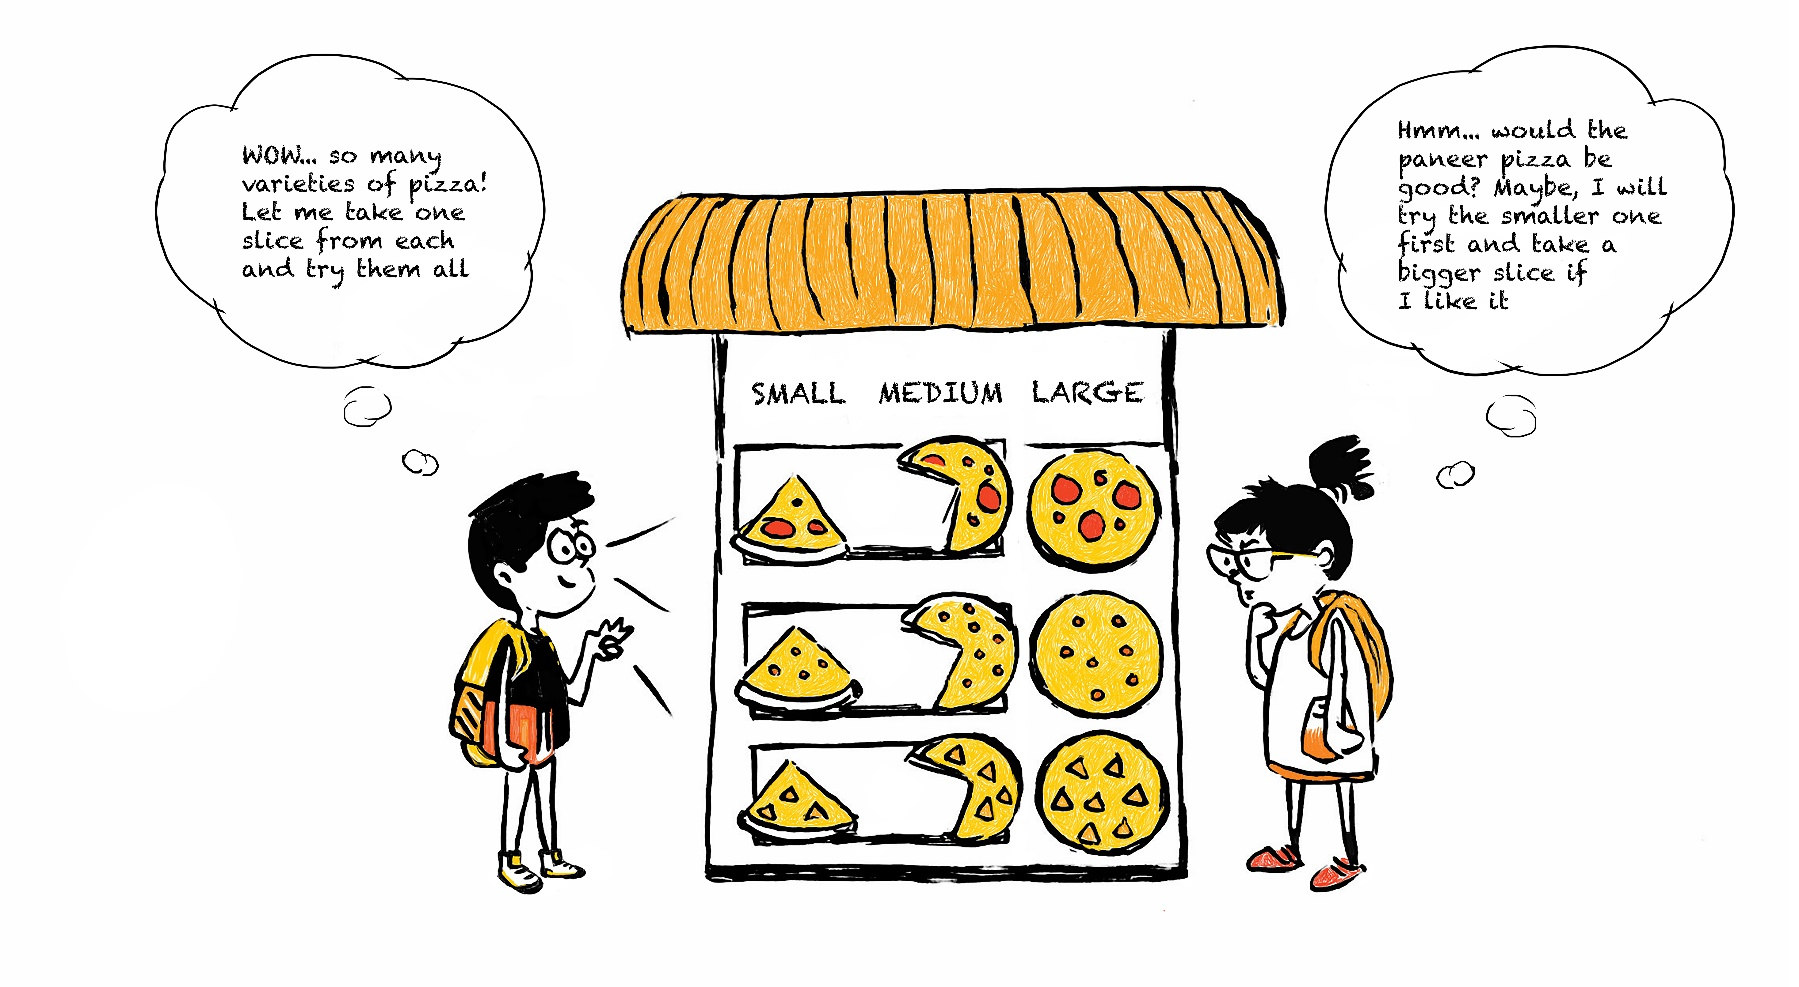
\includegraphics[height=7cm]{./parts/fractal-pizza}
%\end{center}

\section{Glossary of Terms }
\begin{itemize}
\item {\bf Credit:} The quantitative measure of recognition given to a course, stated in semester hours. Typically, a theory course running for a full a semester with three contact hours per week would be 3 credits. Similarly, a lab course with the same number of contact hours would be 2 credits.  
\item {\bf Major:} The primary set of discipline-specific coursework pertaining to the student’s department/discipline  
\item {\bf Minor:} Additional basket of coursework done from a discipline different from the student’s original discipline (and would also find mention in the final degree)
Honors: Additional basket of coursework done in the same discipline as the student’s original discipline (and would also find mention in the final degree)
\item {\bf Double Major:} Coursework pertaining to two departments/disciplines and leading to two separate degrees.
\item {\bf Additional Course:} An additional course taken by the student over and above the minimum credit requirements of the degree. 
Pre-requisite: The preliminary requirement, usually successful completion of another course, that must be met before a course can be taken.
\item {\bf Elective:} Course chosen by the student and which would form part of his/her degree requirements. 
\item {\bf Free Elective:} A course of the student’s choice, to be selected from the any department (subject to meeting the pre-requisites) 
\item {\bf Core Elective:} A course of the student’s choice, to be selected from the same department (or offered by a different department, but identified as "core" by one's department)
\item {\bf LA/CA Elective:} A course of the student’s choice, to be selected from the Liberal Arts and Creative Arts category 
\item {\bf Science Elective:} A course of the student’s choice, to be selected from the Maths, Physics \& Chemistry list of courses
\item {\bf Fractal Segment:} The part or duration of a semester in which a particular course is offered
\end{itemize}

\section{Course Numbering Scheme}
Each course is denoted by a course number consisting of two letters followed by four numerals.
\begin{center}
    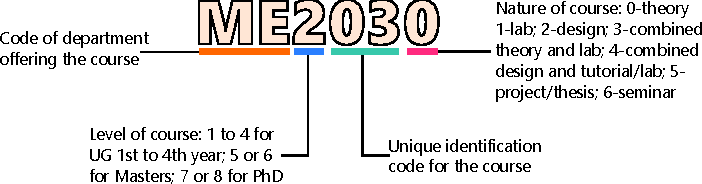
\includegraphics[width=0.8\textwidth, angle=0]{./parts/code-explain.pdf}
%    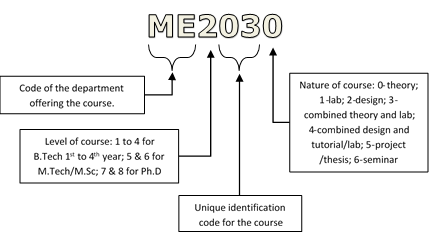
\includegraphics[height=4.5cm]{./parts/course-code}
\end{center}


\section{Fractal Segments}
In the fractal system, a semester is divided into six segments. Each segment is approximately 2.5 to 3 weeks in duration. Every fractal course is accompanied by a two-digit segment number indicating the duration of the course. The first number denotes the segment in which a course will begin and the second number the segment in which it will be completed. For example, Segment 34 means, a particular course will begin in segment-3 and finish at the end of segment-4. Typically, a course running for full the semester (i.e., all six segments) would be 3-credits; so each segment will be equivalent to 0.5 credit. Accordingly, the credit of a course will be decided, based on its segment data. For example, if the segment of a course is 56, it implies that the course will be running in two segments (5 \& 6). Hence, it will be $0.5 \times 2 = 1$ credit. 

\begin{center}

\includegraphics[width=0.3\textwidth]{./parts/segment-explain.pdf}

\begin{tabular}{|c|c|c|c|c|c|c|}
    \hline
    & \multicolumn{6}{|c|}{SEMESTER} \\ \hline
    SEG CREDITS & 1 & 2 & 3 & 4 & 5 & 6 \\ \hline
    0.5 & \multicolumn{1}{|c|}{11}& \multicolumn{1}{|c|}{22}& \multicolumn{1}{|c|}{33}& \multicolumn{1}{|c|}{44}& \multicolumn{1}{|c|}{55}& \multicolumn{1}{|c|}{66} \\ \hline
    1.0 &\multicolumn{2}{|c|}{12}& \multicolumn{2}{|c|}{34} & \multicolumn{2}{|c|}{56} \\ \hline
    1.5 &\multicolumn{3}{|c|}{13}& \multicolumn{3}{|c|}{46} \\ \hline
    2.0 &\multicolumn{4}{|c|}{14}& \hspace{2mm} & \hspace{2mm}  \\ \hline
    2.0 & \hspace{2mm} & \hspace{2mm} & \multicolumn{4}{|c|}{36} \\ \hline
    3.0 &\multicolumn{6}{|c|}{16} \\ \hline
\end{tabular}
\end{center}


\newpage

